\documentclass[a4paper,11pt]{article}

\usepackage{amsmath}
\usepackage{amssymb}
\usepackage{graphicx}
\usepackage{epstopdf}
\epstopdfsetup{update}

\newcommand{\ba}{\begin{array}}
\newcommand{\ea}{\end{array}}

\newcommand{\bea}{\begin{eqnarray}}
\newcommand{\eea}{\end{eqnarray}}

\newcommand{\bc}{\begin{center}}
\newcommand{\ec}{\end{center}}

\newcommand{\ds}{\displaystyle}

\newcommand{\bt}{\begin{tabular}}
\newcommand{\et}{\end{tabular}}

\newcommand{\bi}{\begin{itemize}}
\newcommand{\ei}{\end{itemize}}

\newcommand{\bd}{\begin{description}}
\newcommand{\ed}{\end{description}}

\newcommand{\bp}{\begin{pmatrix}}
\newcommand{\ep}{\end{pmatrix}}

\newcommand{\pd}{\partial}
\newcommand{\sech}{\mbox{sech}}

\newcommand{\cf}{{\it cf.}~}

\newcommand{\ltwo}{L_{2}(\mathbb{R}^{2})}
\newcommand{\smooth}{C^{\infty}_{0}(\mathbb{R}^{2})}

\newcommand{\br}{{\bf r}}
\newcommand{\bk}{{\bf k}}
\newcommand{\bv}{{\bf v}}

\newcommand{\gnorm}[1]{\left|\left| #1\right|\right|}
\newcommand{\ipro}[2]{\left<#1,#2 \right>}

\title{Evolution of Narrow-Band Spectra in Deep-Water Constant Vorticity Flows}
\author{Christopher W. Curtis and Mackensie Murphy}
\date{}
\begin{document}
\maketitle
\section*{Introduction}
There is now a relatively wide range of literature which shows that nonlinear instabilities, in particular the modulational instability (MI), are responsible for significant modifications to the statistical properties of water waves; see \cite{dysthe2,dysthe3,onorato,thomas2012nonlinear} among others.   These results have significant impact on the understanding of deep-water rogue wave formation among other oceanographic phenomena.  However, much of our understanding around MI relies on highly idealized assumptions which cannot be expected to hold in natural settings.  In particular, most understandings of MI rely on looking at the stability of perturbations to carrier waves at essentially a fixed wave number.  To address this shortcoming, in a now seminal paper, \cite{alber} analytically studied families of perturbations of wave packets with narrow, but non-zero, spectral width around a central wave number.  An analytic critierion determining when modulational instability (MI) is either manifested or supressed depending on this spectral width, now refered to as a Benjamin--Feir index (BFI) was derived.  The results in \cite{alber} were confirmed numerically in \cite{dysthe2,dysthe3} by examing the mean properties associated with ensembles of initial conditions.  

However, many physical effects were ignored in the derivation and verification of the results described above. In particular, vorticity was not taken into account, thereby ignoring a central mechanism for the transfer of energy across length scales in oceanic flows.  Thus, building on the work in \cite{thomas2012nonlinear} and \cite{curtis8}, we numerically explore the BFI condition derived in \cite{alber}, focusing in particular on the impact that vorticity plays in controlling the effective width for the onset of MI.  Moving beyond just examining the properties of the nonlinear Schr\"{o}dinger equation (NLSE) with vorticity, we look at the statistical properties of solutions to a higher-order model, the vor-Dysthe equation (VDE) derived in \cite{curtis8}.  As shown in \cite{onorato}, the higher-order terms associated with the Dysthe equation can have significant impacts on the statistics of the waves, so it is a nontrivial question to examine how the vorticity interacts with these higher-order nonlinearities.  

Using our simulations, and as predicted in effect by the results in \cite{curtis8}, we show that we can exacerbate or suppress MI by changing the direction in which the constant vorticity shear profile moves relative to the propagating surface waves.  Using ensembles of initial conditions for a given choice of spectral width, we see that both the NLSE and VDE exhibit either the MI or supression thereof predicted by the BFI as derived in \cite{alber}.  However, as we show, starting from Gaussian initial conditions, the NLSE generates essentially Gaussian results.  Moreover, it is incapable of shifting means, and thus is clearly of limited utility in describing realistic wave fields.  In contrast, our results show that the VDE is able to capture non-Gaussian effects and allows for shifts in the mean relative to the distribution of initial conditions.  

A particularly interesting consequence of looking at wave packets is that the BFI condition gives one an estimate of what class of wavetrains would be stable given a particular shear profile.  Thus, if one supposes that only stable profiles are physically observable, then the results in this paper give an indication of what wave trains one is most likely to see in oceanographic contexts.  

\section*{Modeling and Stability Theory}
We examine the unsteady nonlinear wave propagation over a constant shear current.  To do this, we assume the fluid velocity has the form
\[
{\bf u} = u({\bf x},t)\hat{{\bf x}} + w({\bf x},t)\hat{{\bf z}} = \omega z\hat{{\bf x}} + \nabla \phi,
\]
where $\phi$ is a harmonic function.  We restrict fluid motion to the $(x,z)$-plane, thereby ignoring transverse variations in the $y$ dimension.   Following standard arguments, e.g.~see \cite{ashton}, the dynamics of the fluid can be determined by solving the free boundary value problem
\begin{align}
\Delta \phi = 0, & & -\infty< z < \eta(x,t), \nonumber \\
\eta_{t} +\left(\omega\eta+\phi_{x}\right)\eta_{x} - \phi_{z} = 0, & & z=\eta(x,t), \label{kine}\\
\phi_{t} + \omega\pd_{x}^{-1}\eta_{t} + \frac{1}{2} \left|{\bf
    u}\right|^{2} + g\eta -
\frac{\sigma}{\rho}\pd_{x}\frac{\eta_{x}}{\sqrt{1+\eta_{x}^{2}}}= 0, &
& z=\eta(x,t), \label{bernou}\\
\lim_{z\rightarrow -\infty} \phi_{z} = 0, \nonumber
\end{align}
where $\eta$ represents the free surface displacement, and $g$, $\rho$, and $\sigma$ represent the acceleration due to gravity, the fluid density, and the coefficient of surface tension respectively.

By choosing a characteristic wave height $a$ and wave length $L$, all quantities can be non-dimensionalized via
\begin{align*}
\tilde{x} = \frac{x}{L}, ~\tilde{z} = \frac{z}{L}, ~ \tilde{t} = \sqrt{\frac{g}{L}}~t, ~\omega = \sqrt{\frac{g}{L}}~\tilde{\omega}, \\
\eta = a \tilde{\eta}, ~ \phi  = a\sqrt{gL}~\tilde{\phi} , ~ \epsilon = \frac{a}{L}.
\end{align*}
By following the AFM approach described in \cite{afm,ashton} and dropping the tildes, the kinematic boundary condition, Equation \eqref{kine}, can be written in terms of surface variables alone via the integro-differential equation
\begin{equation}
\int_{\mathbb{R}}dx~e^{-ikx}e^{\epsilon|k|\eta}\left(\eta_{t} +
  \epsilon \omega \eta \eta_{x} + i \mbox{sgn}(k)Q \right) = 0, ~
k\neq 0,
\label{kine2}
\end{equation}
where $Q=q_{x}$, $q(x,t) = \phi(x,\eta(x,t),t)$.  By integrating over $\mathbb{R}$, we are assuming that both $\eta$ and $Q$ decay to zero sufficiently rapidly in the far field.  We can also readily derive a nearly identical expression on domains periodic in the horizontal variable $x$, in which case Equation \eqref{kine2} becomes
\begin{equation}
\int_{-L_{p}/2}^{L_{p}/2}dx~e^{-ikx}e^{\epsilon|k|\eta}\left(\eta_{t} +
  \epsilon \omega \eta \eta_{x} + i \mbox{sgn}(k)Q \right) = 0, ~ k = \frac{2\pi m}{L_{p}}, ~ m\in \mathbb{Z}\backslash{0},
\label{integro1per}
\end{equation}
where $L_p$ is the spatial period.  Throughout the remainder of this section we only present results over the real line, $\mathbb{R}$, since identical results can be derived for the periodic case.
Lastly, we note that if in Equation \eqref{kine2} we approach $k=0$ from both the left and the right, we get the equations
\[
\int_{\mathbb{R}}dx \left(\eta_{t} + i Q \right) = 0, ~ \int_{\mathbb{R}}dx \left(\eta_{t} - i Q \right) = 0.
\]
Thus we get the identities
\begin{align}
\pd_{t}\int_{\mathbb{R}} dx ~\eta(x,t) & = 0, \label{zavsurf}\\
\int_{\mathbb{R}} dx ~Q(x,t) & = 0. \label{zavpot}
\end{align}

\begin{multline}
\int_{\mathbb{R}}dx~e^{-ikx}\left(1 + \epsilon |k|\eta + \frac{\epsilon^{2}|k|^{2}\eta^{2}}{2} + \frac{\epsilon^{3}|k|^{3}\eta^{3}}{6}\right)\left(\eta_{t} + i \mbox{sgn}(k)Q \right) \\
+ \epsilon \omega \int_{\mathbb{R}}dx~e^{-ikx}\left(1 + \epsilon |k|\eta + \frac{\epsilon^{2}|k|^{2}\eta^{2}}{2}\right) \eta \eta_{x} = 0.
\label{integro1}
\end{multline}
Transforming into surface variables and Taylor expanding Equation \eqref{bernou}, Bernoulli's equation, up to $\mathcal{O}(\epsilon^3)$ gives
\begin{multline}
Q_{t} + \omega \eta_{t} + \eta_{x} - \tilde{\sigma}\eta_{xxx} + \frac{\epsilon}{2}\pd_{x}\left(-\eta_{t}^{2} + (Q+\omega \eta)^{2} \right)\\
+ \epsilon^{2}\pd_{x}\left( \frac{3}{2}\tilde{\sigma}\eta_{x}^{2}\eta_{xx} - \eta_{t}\eta_{x} \left(Q  + \omega \eta \right) \right) - \frac{\epsilon^{3}}{2}\eta_{x}^{2}\left((\omega\eta+Q)^{2}-\eta_{t}^{2}\right) = 0,
\label{berexp}
\end{multline}
where the reciprocal of the Bond number, $\tilde{\sigma}$, is given by
\[
\tilde{\sigma} = \frac{\sigma}{\rho g L^2}.
\]
We note that we have tacitly assumed $\omega = \mathcal{O}(1)$.  In physical terms, this implies that $\omega$ is comparable to the natural time scale of this problem, $\sqrt{L/g}$.  If we were to assume $\omega$ were of larger magnitude, the problem would no longer be weakly nonlinear and would be much less amenable to asymptotic analysis.  Therefore, throughout the remainder of the paper, we assume that the vorticity is not too large.

%By expanding Equation \eqref{integro1} and taking inverse Fourier transforms, we can derive the first three terms of the corresponding Dirichlet-to-Neumann Operator (DNO) expansion, so that we find
%\begin{equation}
%\eta_{t} = G_{0}Q + \epsilon G_{1}Q + \epsilon^{2}G_{2}Q,
%\label{dnoexp}
%\end{equation}
%where
%\begin{align*}
%G_{0}Q = & -\mathcal{H}Q\\
%G_{1}Q = & \mathcal{H}\pd_{x}\left(\eta G_{0}Q\right) - \pd_{x}\left(\eta Q + \frac{\omega}{2}\eta^{2}\right)\\
%G_{2}Q = & \mathcal{H}\pd_{x}\left(\eta G_{1}Q\right) + \frac{1}{2}\pd_{x}^{2}\left(\eta^{2}G_{0}Q \right) + \pd_{x}^{2}\mathcal{H}\left(\frac{1}{2}\eta^{2}Q + \frac{\omega}{3}\eta^{3}\right), 
%\end{align*}


%Using the DNO expansion in Equation \eqref{dnoexp}, we can rewrite Equation \eqref{berexp} an an evolution equation for $Q_{t}$, thereby giving us a closed system in terms of surface variables alone.  The system of equations given by Equations \eqref{dnoexp} and \eqref{berexp} we denote as the Full-Euler Equations (FEEs).  

As is well known by now, in non-dimensional variables, we can model the evolution of a relatively small free-fluid surface over infinitely-deep water $z=\epsilon \eta(x,t)$ via the expansion 
\begin{multline*}
\eta(x,t) = \eta_{1}(\xi,\tau)e^{i\theta(x,t)} + \eta^{\ast}_{1}(\xi,\tau)e^{-i\theta(x,t)}\\
+ \epsilon\left(\eta_{0}(\xi,\tau) + \eta_{2}(\xi,\tau)e^{2i\theta(x,t)} + \eta^{\ast}_{2}(\xi,\tau)e^{-2i\theta(x,t)}\right) + \mathcal{O}\left(\epsilon^{2} \right)
\end{multline*}
where $\tau = \epsilon^{2}t$, $\xi = \epsilon(x+c_{g}t)$, and $\theta(x,t) = k_{0}x + \Omega(k_{0},\omega)t$, where the linear dispersion relationship $\Omega(k_{0},\omega)$ is given by
\[
\Omega(k_{0},\omega) = \frac{1}{2}\left(s\omega \pm \sqrt{\omega^{2} + 4|k_{0}|\left(1+\tilde{\sigma}k_{0}^{2}\right)} \right).
\]
Here, $s = \mbox{sgn}(k_{0})$, $\omega$ is the non-dimensionalized magnitude of the vorticity of the flow, and $\tilde{\sigma}$ is the surface tension.  

To describe the evolution of the slowly evolving envelope $\eta_{1}(\xi,\tau)$, we use two asymptotically accurate models.  The first model is the the nonlinear Schr\"{o}dinger equation (NLSE) derived in \cite{curtis8}, though see also \cite{thomas2012nonlinear}, given by 
\[
i\pd_{\tau}\eta_{1} + \alpha_{d}\pd_{\xi}^{2}\eta_{1} + \alpha_{nl}\left|\eta_{1} \right|^{2}\eta_{1} = 0, 
\]
where 
\begin{align*}
c_{g} = & \frac{1+3\tilde{\sigma}k_{0}^{2}}{2s\Omega - \omega},\\
\alpha_{d}(k_{0},\omega) = & \frac{(c^2_{g} - 3|k_{0}|\tilde{\sigma})}{2\Omega-s\omega},\\
\alpha_{nl}(k_{0},\omega) = & \frac{k_{0}\left( sk_{0}^{3}\left(8 + \tilde{\sigma}k_{0}^{2} + 2(\tilde{\sigma}k_{0}^{2})^{2}\right) + \omega \alpha_{v}\right)}{\left(2s\Omega -\omega\right)(1+c_{g}\omega)\left(4\Omega^2-s(2k_{0}(1+4\tilde{\sigma}k_{0}^{2})+2\omega\Omega)\right)}.
\end{align*}

However, the NLSE is a relatively low-order model known to be only of limited use in real-world modeling situations.  A more robust model, following the work in \cite{dysthe1}, is found by going to the next higher order in $\epsilon$, giving us the 
\begin{multline}
(\omega-2s\Omega)\pd_{\tau}\eta_{1} + i(c_{g}^{2}s-3k_{0}\tilde{\sigma})\pd_{\xi}^{2}\eta_{1} + 2i\epsilon s c_{g}\pd^{2}_{\xi\tau}\eta_{1} - \epsilon\tilde{\sigma} \pd^{3}_{\xi}\eta_{1} + i\epsilon^{2}c_{h}\pd_{\xi}^{4}\eta_{1} \\
- i \alpha_{nl}(\omega-2s\Omega)\left|\eta_{1}\right|^{2}\eta_{1}
+ \epsilon \tilde{\alpha}_{1}\left|\eta_{1}\right|^{2}\pd_{\xi}\eta_{1}
+ \epsilon\tilde{\alpha}_{2}\eta_{1}^{2}\pd_{\xi}\eta^{\ast}_{1} +
\epsilon i\tilde{\alpha}_{3}\eta_{1}\mathcal{H}\pd_{\xi}\left|\eta_{1}\right|^{2}= 0.
\label{dysthe}
\end{multline}
where $\mathcal{H}$ denotes the Hilbert transform so that 
\[
\mathcal{H}f = \frac{1}{2\pi}\int_{\mathbb{R}}dk~ e^{ikx}  i\mbox{sgn}(k) \hat{f}(k),
\]
where $\hat{f}(k)$ is the Fourier transform of $f(x)$ defined by
\[
\hat{f}(k) = \int_{\mathbb{R}}dx~ e^{-ikx}f(x).
\]
We call Equation \eqref{dysthe} the Vor-Dysthe (VD) equation.  Details of its derivation can be found in \cite{curtis8}, though we note a difference in this work with that in \cite{curtis8}.  In this work, we found the inclusion of the higher-order dispersion associated with the coefficient $c_{h}$, given by
\[
c_{h} = 2sc_{g}(2sc_{g}\alpha_{d}+\tilde{\sigma})/(\omega-2s\Omega) - s\alpha_{d}^{2},
\]
was necessary to remove artificial numerical instabilities.  Similar issues with Dysthe like equations have been noted in (add appropriate citation).  Moreover, the coefficients $\tilde{\alpha}_{j}$ are readily derived, but their forms are cumbersome and thus we omit explicitly writing them for the sake of readability.  

To generate simulations, we start both the NLSE and VDE from the same collection of $2L$ periodic-initial conditions
\[
\eta_{1}(\xi,0) = \epsilon_{rms}\sqrt{\frac{\delta \tilde{k}}{\sigma\sqrt{\pi}}} \sum_{k=-K+1}^{K}e^{-\tilde{k}^{2}/2\sigma^{2}}e^{i\theta_{k}}e^{i\tilde{k}\xi}, ~ \tilde{k} = \frac{\pi k}{L},
\]
where $\delta \tilde{k}=\pi/L$ and the phases $\theta_{k}$ are randomly chosen uniformly between $0$ and $2\pi$.  We can then readily show that, for $L\gg 1$, 
\[
\epsilon_{rms} \approx \overline{\left|\eta_{1}\right|^{2}}^{1/2},
\]
where $\overline{()}$ denotes the ensemble average.  In our coordinates then, the work in \cite{alber} and later confirmed in \cite{dysthe2} shows that for the NLSE the MI is suppressed for spectral widths $\sigma$ such that 
\[
\sigma \geq \sigma_{c}, ~ \sigma_{c} = \epsilon_{rms}\sqrt{\frac{2\alpha_{nl}}{\alpha_{d}}}
\]
This work has helped motivate defining this parameter as the Benjamin--Feir Index (BFI), which has been shown to be a critical parameter to understanding the statstical properties of nonlinear free-surface flows; see \cite{onorato, thomas2012nonlinear}.
\section*{Results}
To understand the relationship between the vorticity $\omega$ and the initial spectral width $\sigma$ of our initial conditions, we generate ensembles of initial conditions and then run these different initial conditions up to $\tau=2$ which corresponds to $t_{f} = 2/\epsilon^{2}$ in the original fast variables.  The domain is $[-50\pi,50\pi]$.  The number of modes is $K = 512$.  The surface tension is $\tilde{\sigma} = 10^{-5}$. We then plot the averaged spectral density $S(k,t_{f};\sigma)$ where 
\[
S\left(k,t_{f};\sigma\right) = \overline{\left( \left|\frac{1}{\epsilon}\hat{\eta}_{1}\left(\frac{k-k_{0}}{\epsilon},1;\sigma \right)\right|^{2}\right)}.
\]
which corresponds to the autocorrelation of the surface profile with respect to space.  Note we have emphasized the dependence on the initial spectral width $\sigma$ for the sake of clarity.  Following the approach in \cite{dysthe2,dysthe3}, by comparing the initial spectral density to that at later times, we can see directly whether MI manifests as significant distortions of the statistics, or if through supression the distributions remain relatively close to one another.  

Throughout our results, we have used a psuedo-spectral method in space coupled with a 4th-order Runge-Kutta scheme using integrating factors in time, with a time step of $dt = 2.5 \times 10^{-3}$.  De-aliasing is implemented via Orszag's `2/3-rule'.  Averaging was done with $N_{e}=512$ ensemble members, thereby ensuring relative averaging errors on the order of about $1\%$.  Throughout this section, we present comparisons of the distributions for particular choices of $\sigma$ while also comparing the mean and standard deviations of the respective distributions so as to get a more quantitative understanding of the differences between the different distributions.  

\subsection*{Strong-Counter Shear: $\omega = -1$}

Motivated by the results in \cite{curtis8}, we anticipate that $\omega=-1$ presents the most case which would allow for the vorticity to have the strongest impact on the BFI condition, which for the parameter choices gives us the BFI $\sigma_{c} \approx 11.9$.  This is borne out by numerical experiment as seen in Figure \ref{fig:meanstdomn1}.  In this case, we see that for the NLSE the BFI condition largely holds.  In particular, we see that while the mean never changes in any significant way from that of the initial distribution, increasing the width $\sigma$ causes the standard deviation of the distribution determined via evolution of the NLSE to collapse onto that of the initial, thereby showing that wider spreads in initial conditions are overall less susceptible to MI.   

\begin{figure}[!ht]
\centering
\begin{tabular}{c}
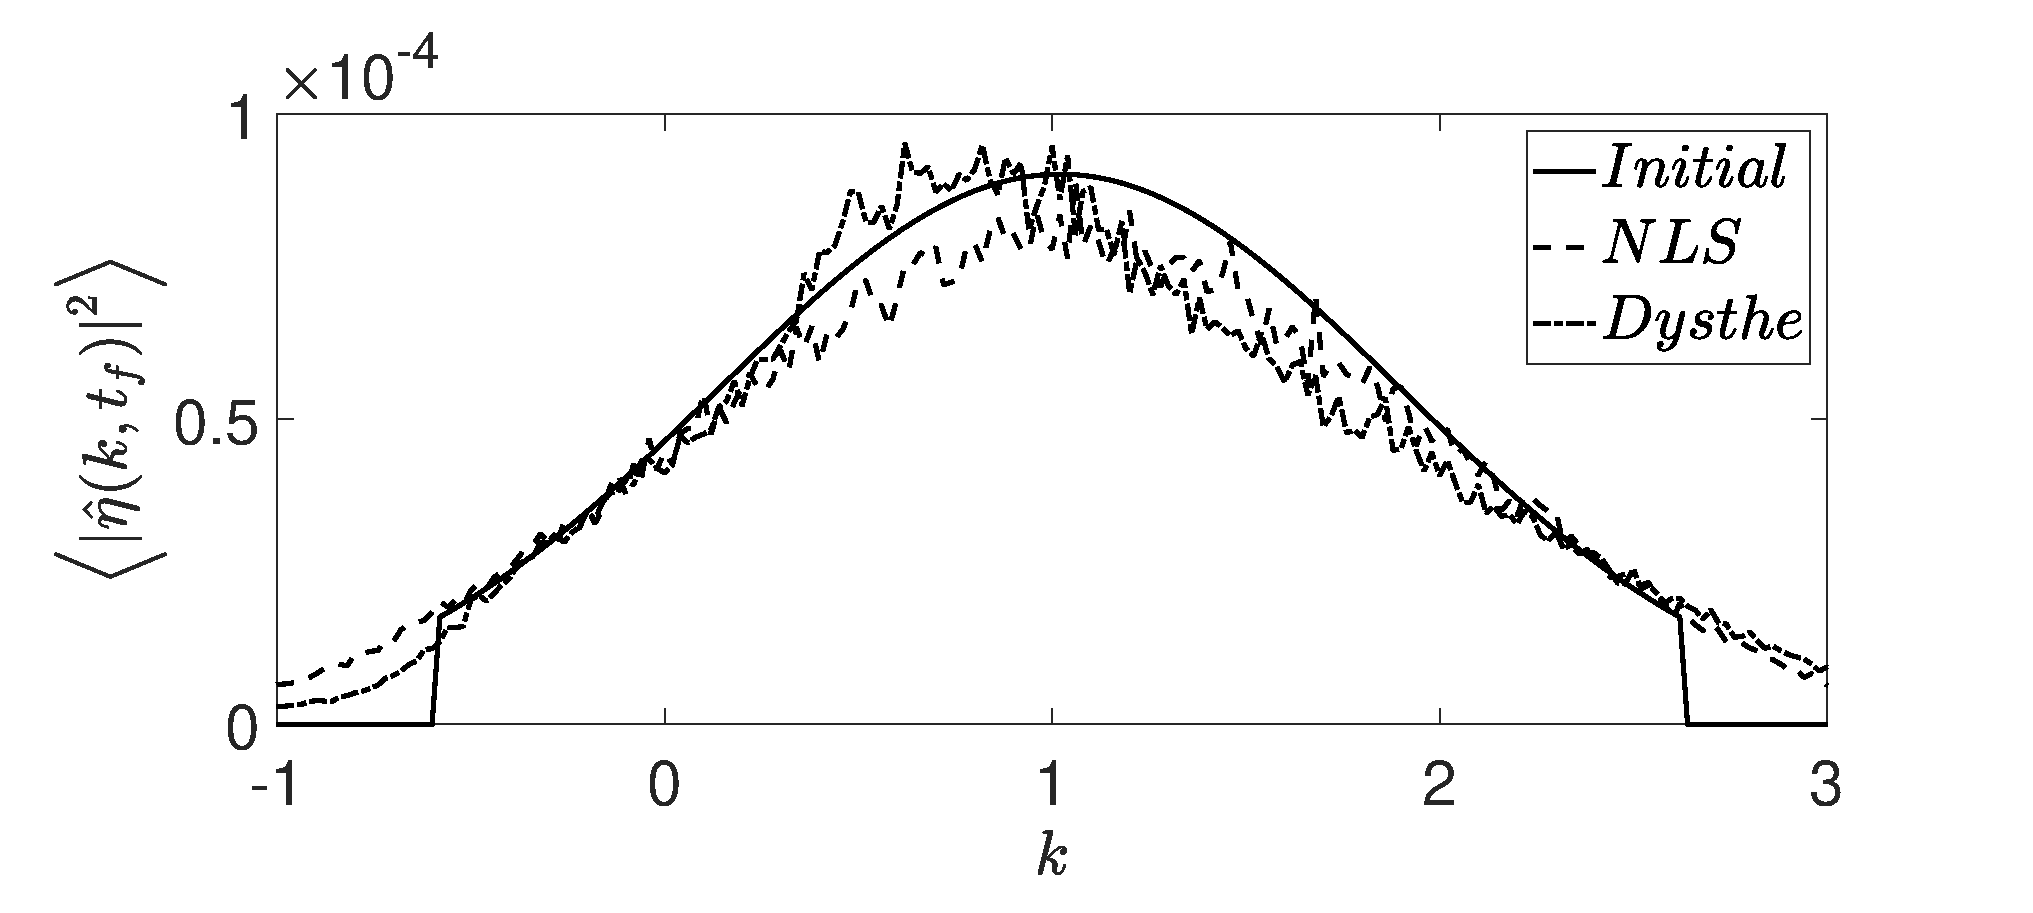
\includegraphics[width=.65\textwidth]{pdf_w_n1_ep_pt1_Nens_512} \\
(a) $\epsilon=.1$\\
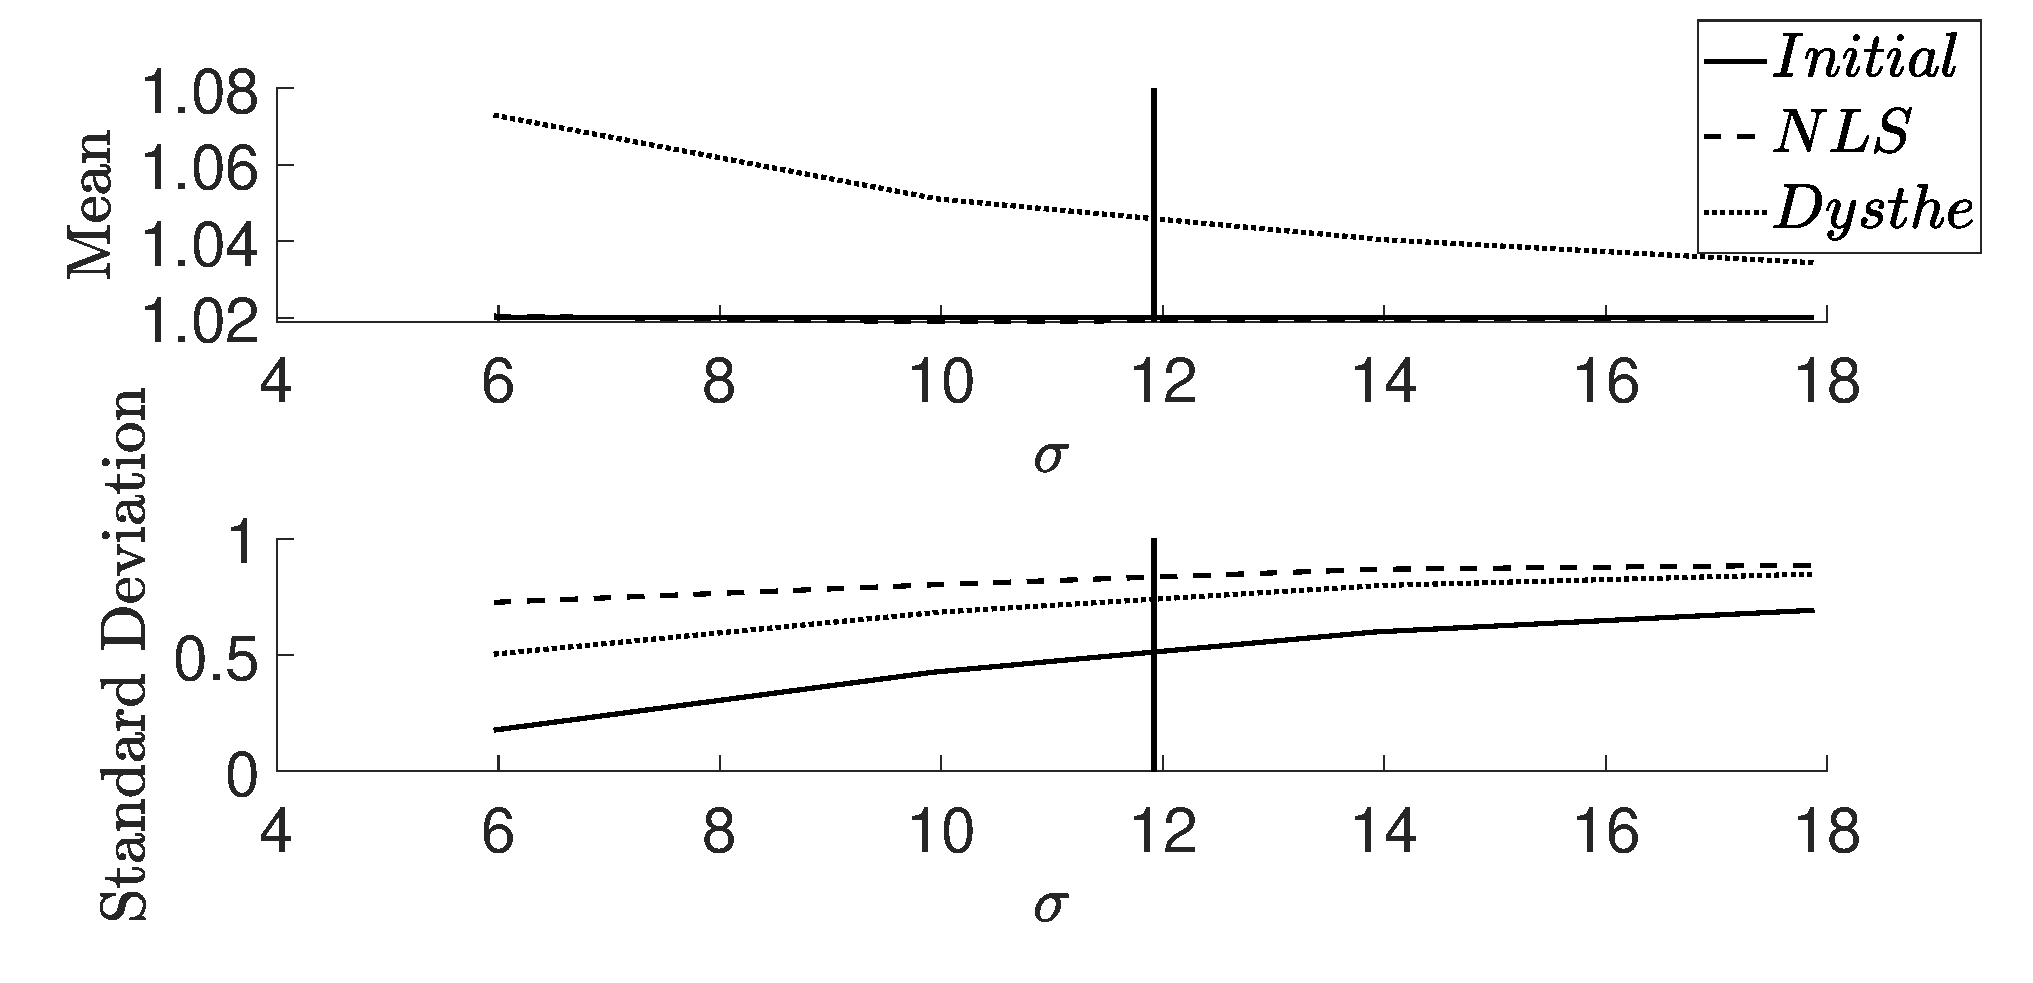
\includegraphics[width=.65\textwidth]{omega_n1_mean_std_plot_ep_pt1}\\
(b) $\epsilon=.1$ \\
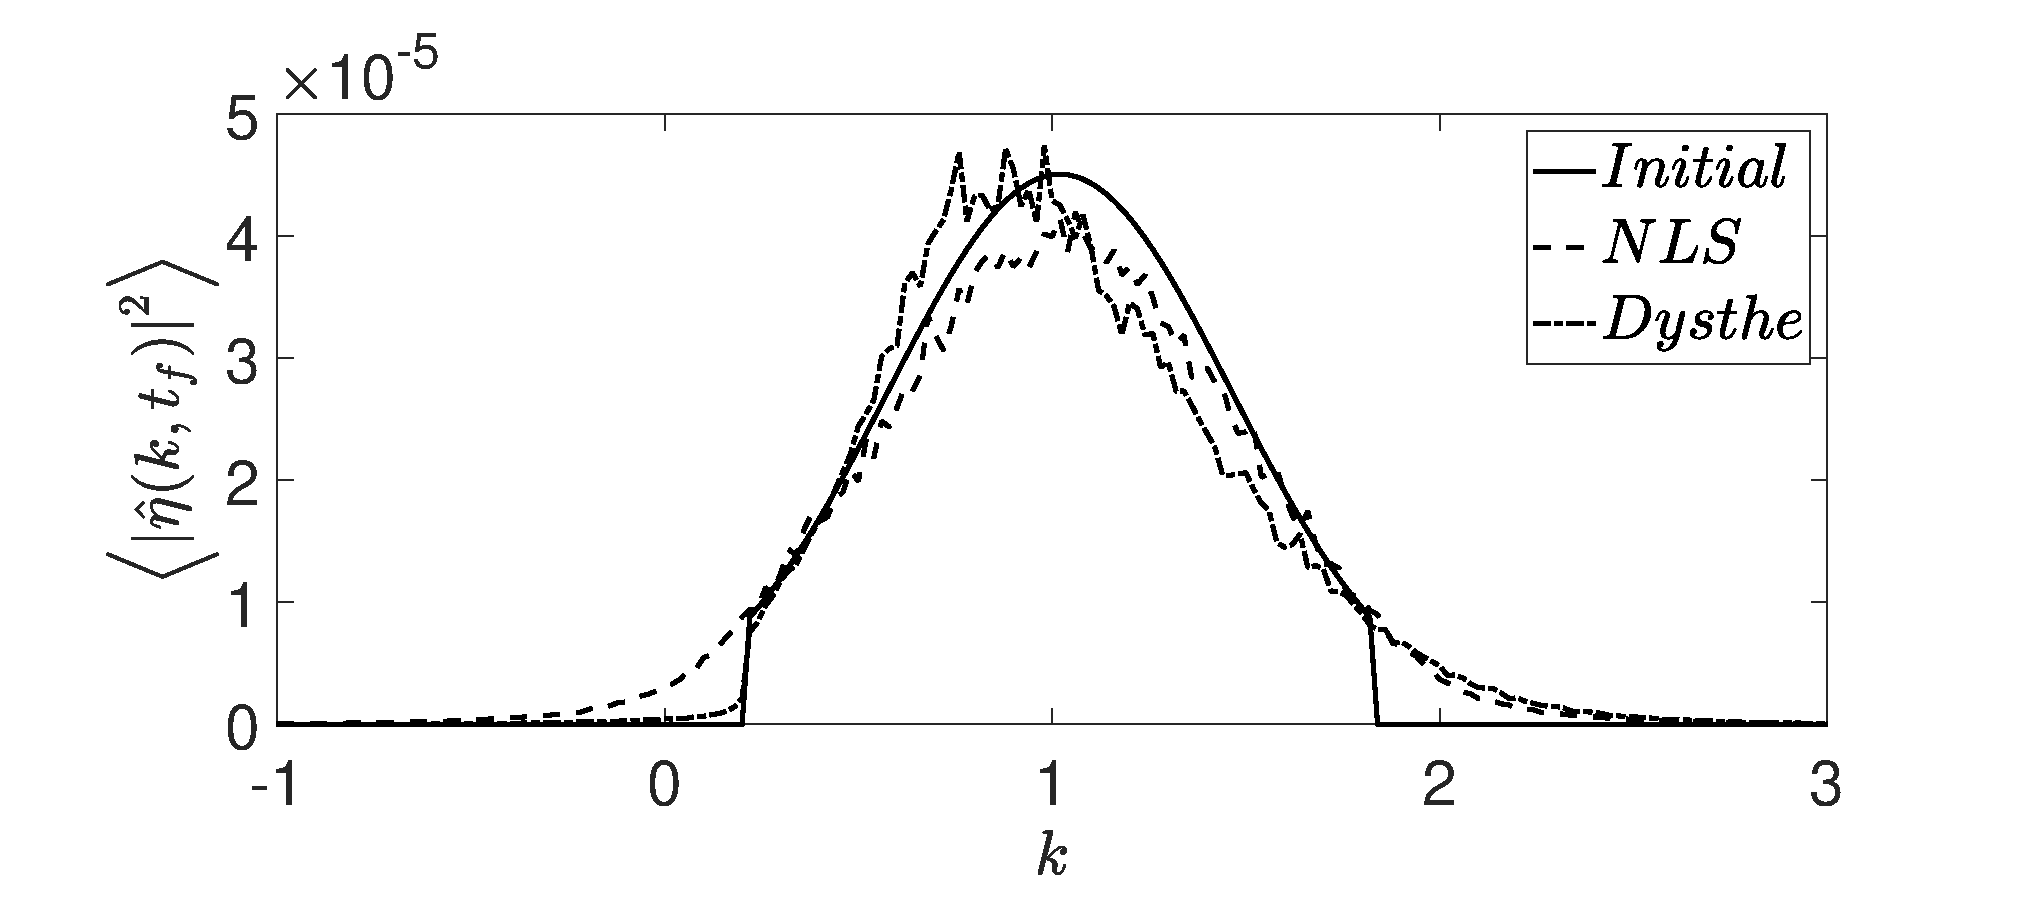
\includegraphics[width=.65\textwidth]{pdf_w_n1_ep_pt05_Nens_512}\\
(c) $\epsilon=.05$ \\
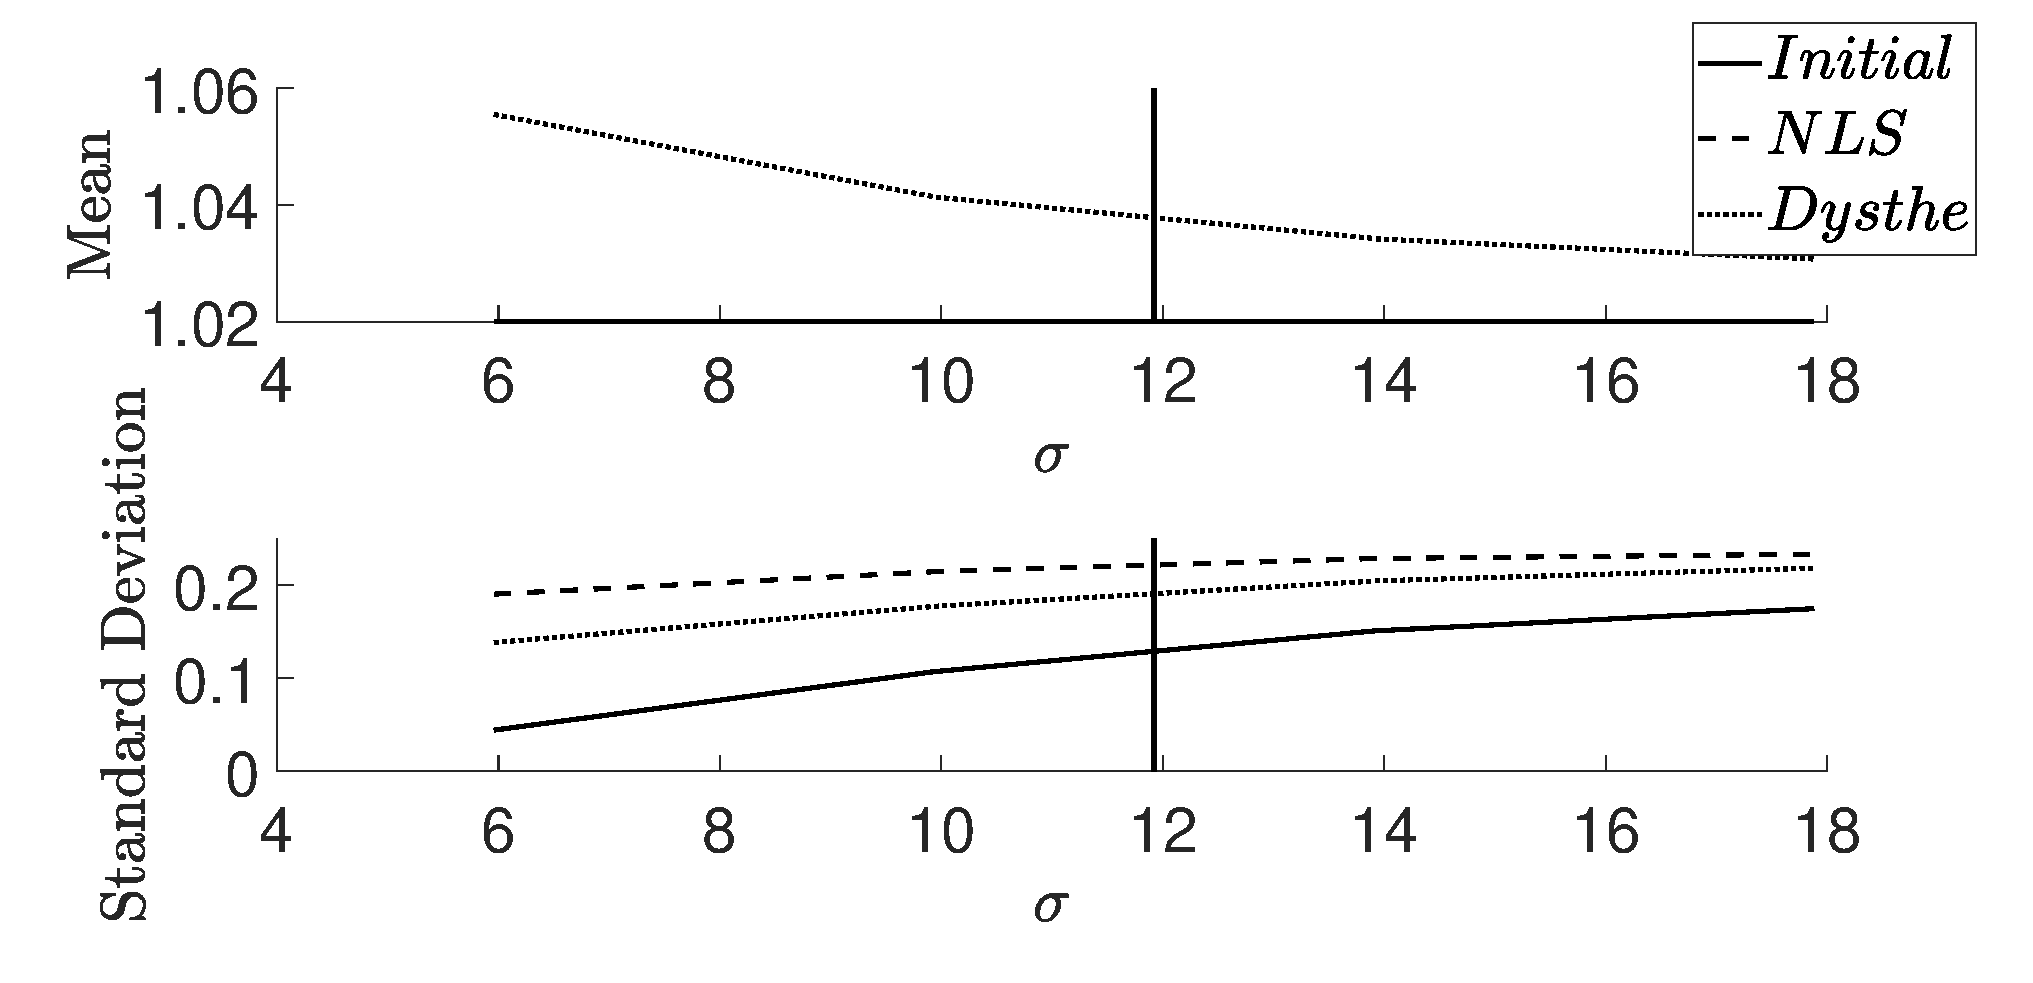
\includegraphics[width=.65\textwidth]{omega_n1_mean_std_plot_ep_pt05}\\
(d) $\epsilon=.05$
\end{tabular}
\caption{For $\omega=-1$, in (a) and (c) plots of the distributions for $\epsilon=.1$ and $\epsilon=.05$ respectively,  with $\sigma=1.05\sigma_{c}$.  In (b) and (d) comparison of the means and standard deviations between the initial averaged spectral density for $\epsilon=.1$ and $\epsilon=.05$ respectively.  The vertical line denotes the spectral width corresponding to the BFI condition.}
\label{fig:meanstdomn1}
\end{figure}

However, the results for the VDE are markedly different.  As seen in Figure \ref{fig:meanstdomn1}, where $\sigma=12$ so that we are just past the BFI threshold,there is clearly a frequency downshift of the central initial peak.  This downshift is less pronounced with decreasing $\epsilon$, but is clearly there nevertheless.  Likewise, noting that the overall mean is rightshifted in Figures \ref{fig:meansdomn1} (b) and (d), we see that the tails of the distributions are skewed in the VDE, in effect adding kurtosis and pushing the final distribution away from the Gaussian initial conditions.  

\subsection*{Vorticity-Free Flow: $\omega = 0$}

Removing vorticity, we see that we essentially recreate the standard BFI, with BFI threshold $\sigma > 5.7$, results for the NLSE.  Again though, the VDE produces markedly different statistical results from the NLS, though to nowhere near as drastic an extent as when $\omega=-1$.  In particular, the bimodality and strong deformation of the profile is notably ameliorated for $\epsilon=.05$; see Figure \ref{fig:meanstdom0}.  Thus in some sense, though not entirely, MI has more or less similar characteristics for both the NLSE and VDE. 

\begin{figure}[!ht]
\centering
\begin{tabular}{c}
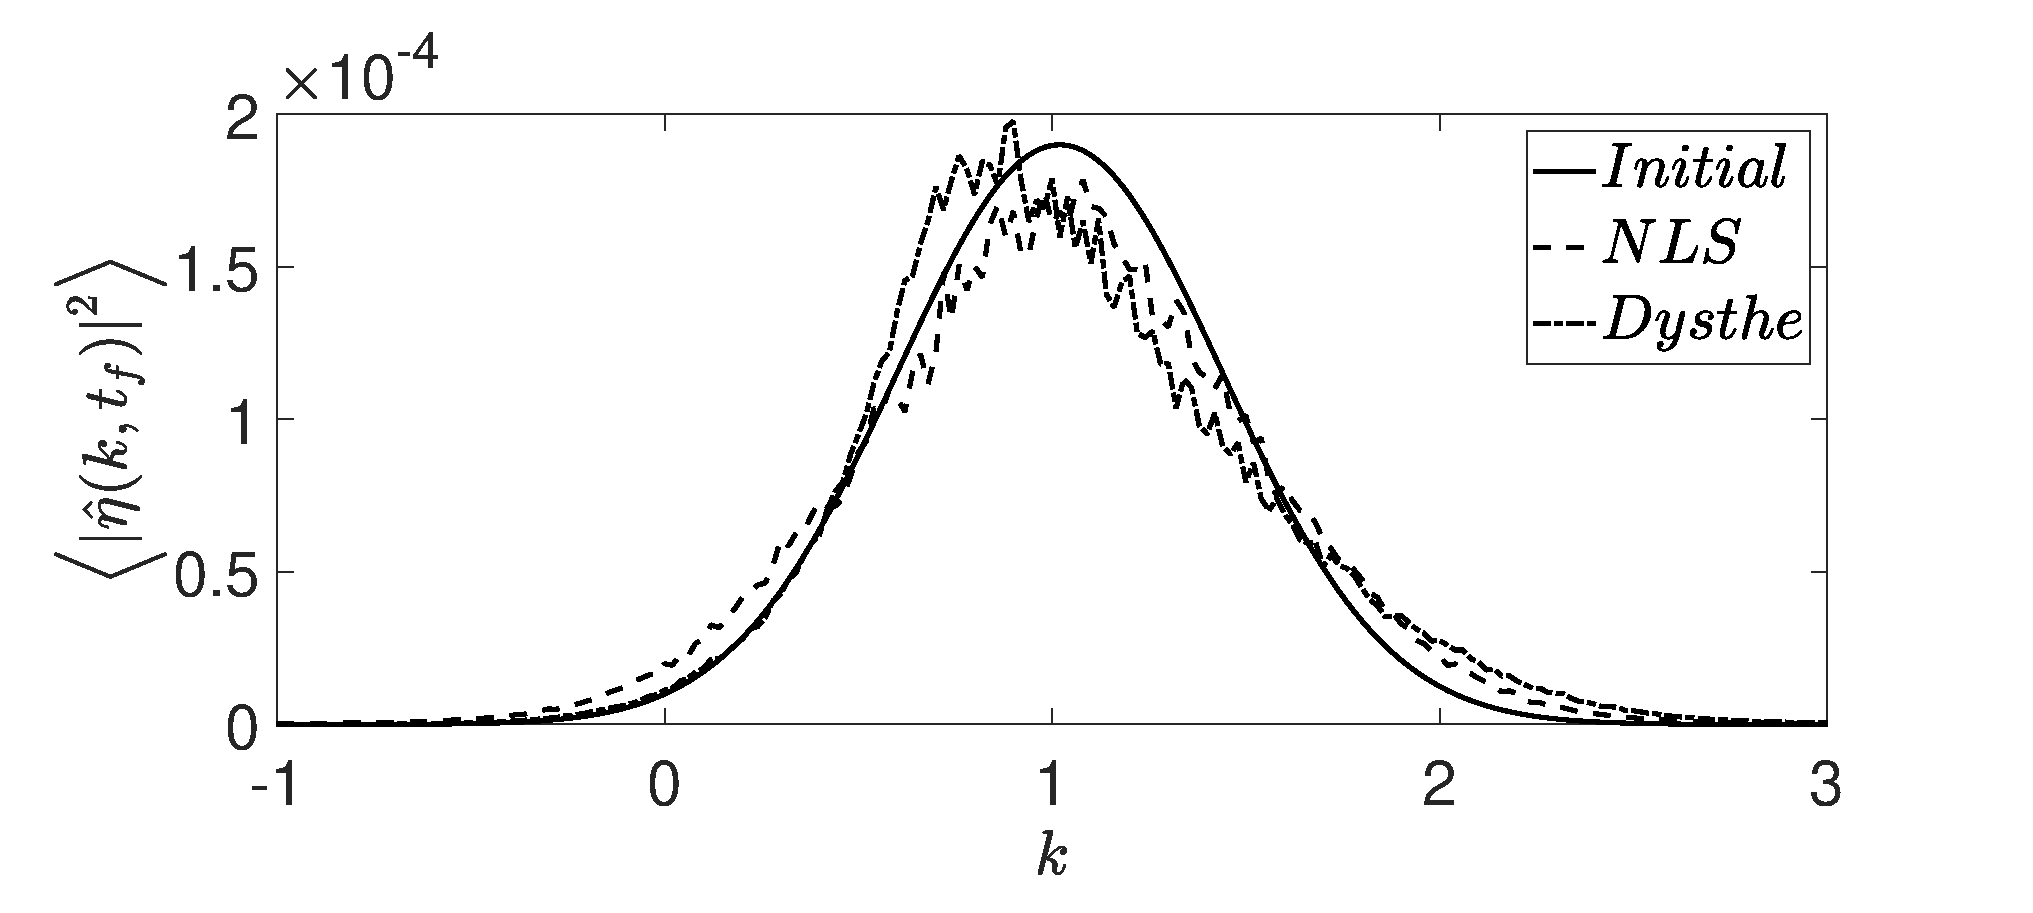
\includegraphics[width=.65\textwidth]{pdf_w_0_ep_pt1_Nens_512} \\
(a) $\epsilon=.1$\\
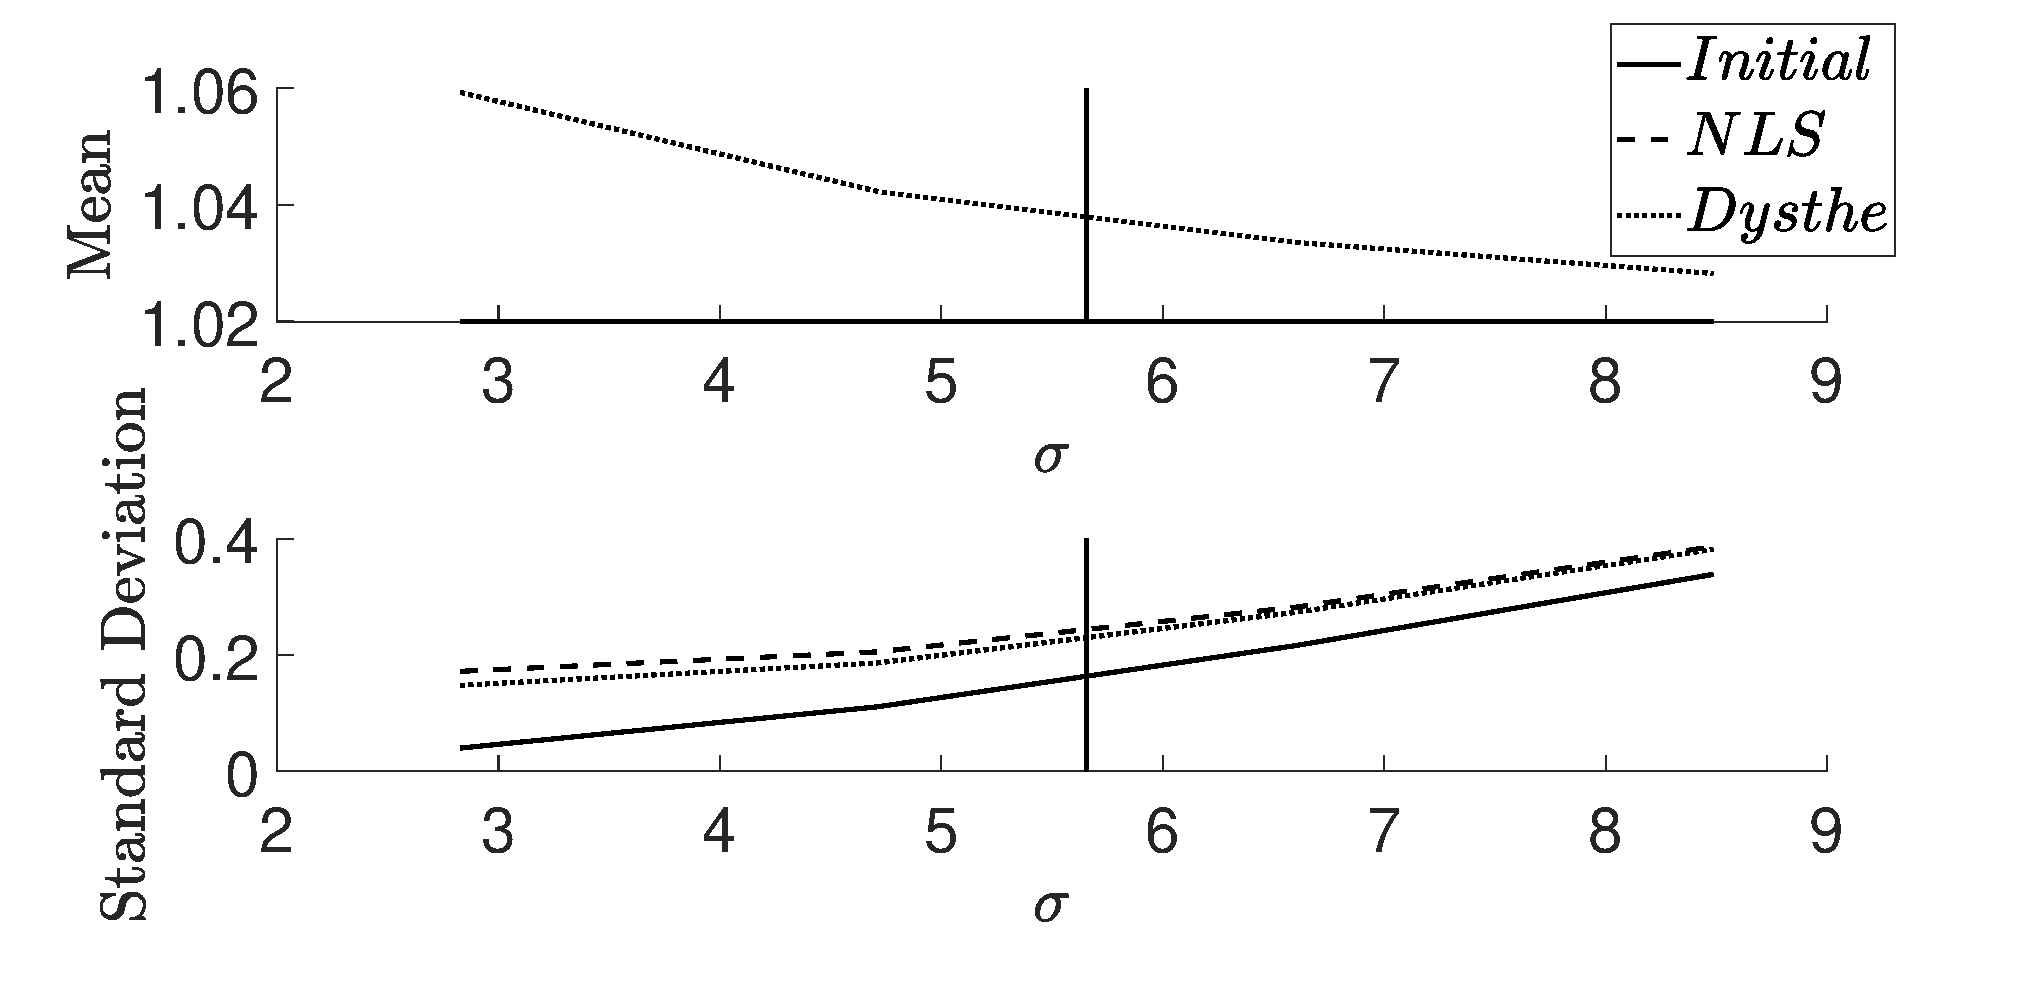
\includegraphics[width=.65\textwidth]{omega_0_mean_std_plot_ep_pt1}\\
(b) $\epsilon=.1$ \\
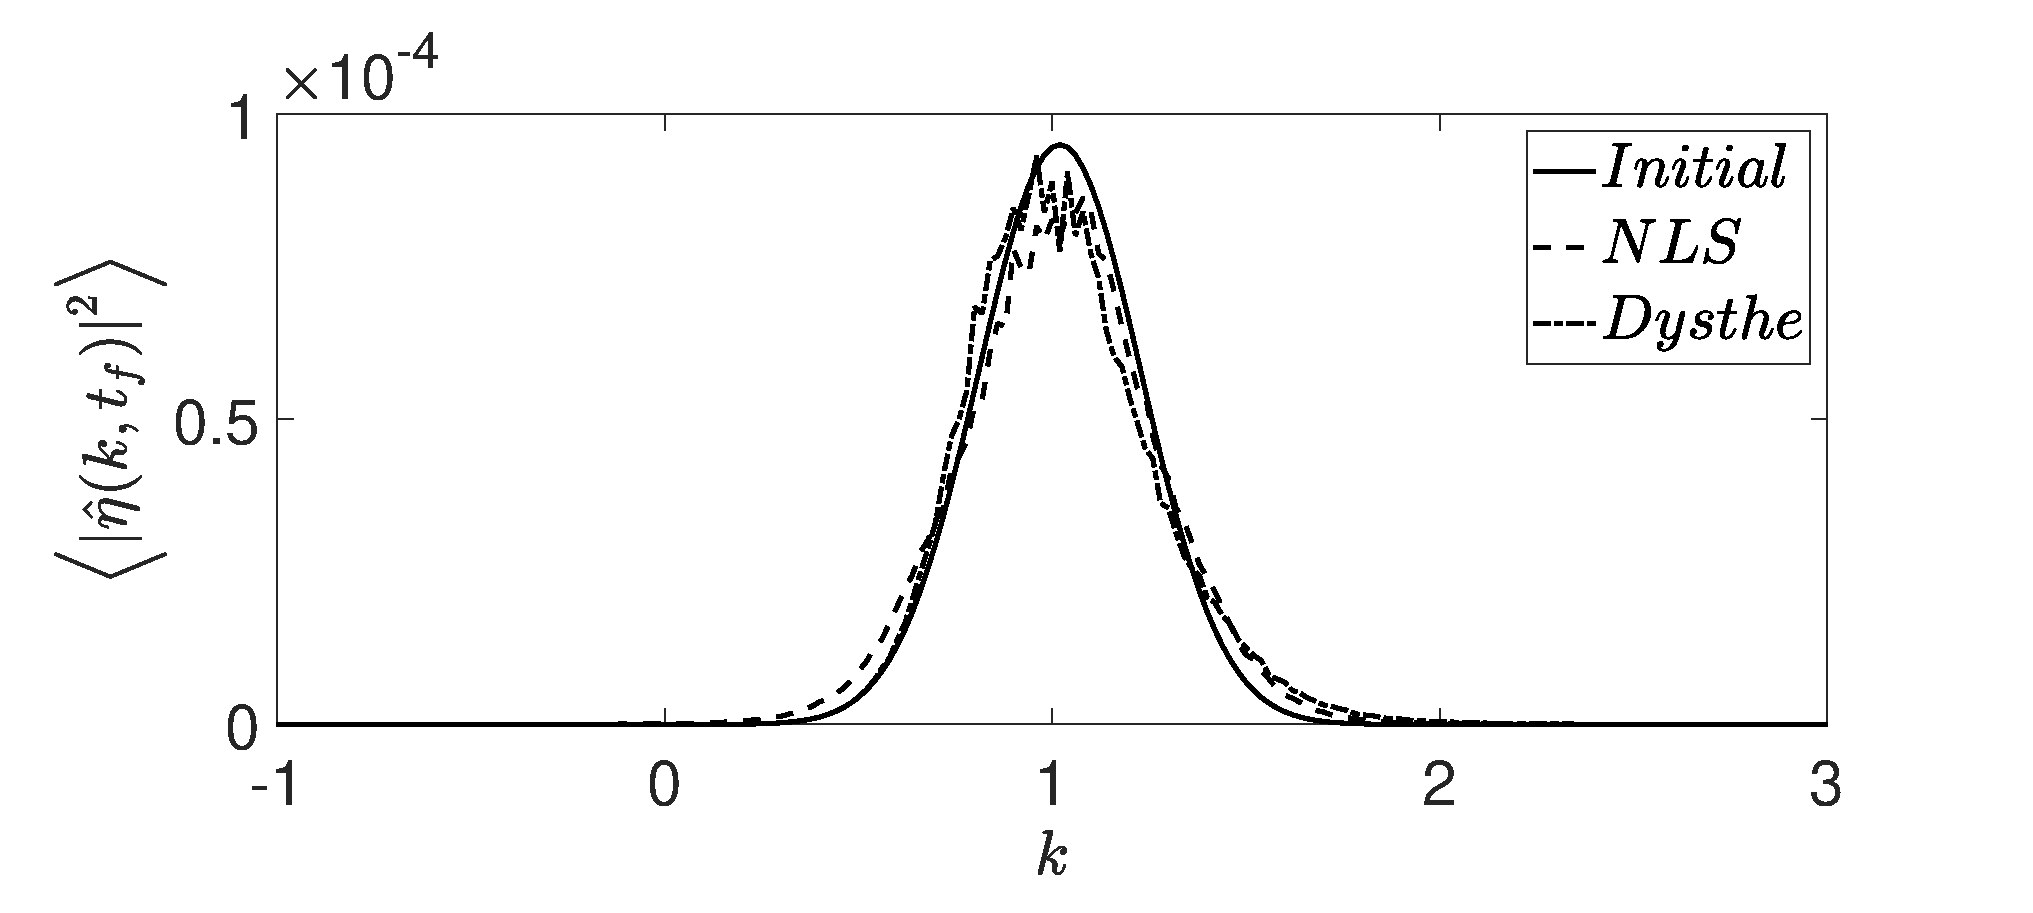
\includegraphics[width=.65\textwidth]{pdf_w_0_ep_pt05_Nens_512}\\
(c) $\epsilon=.05$ \\
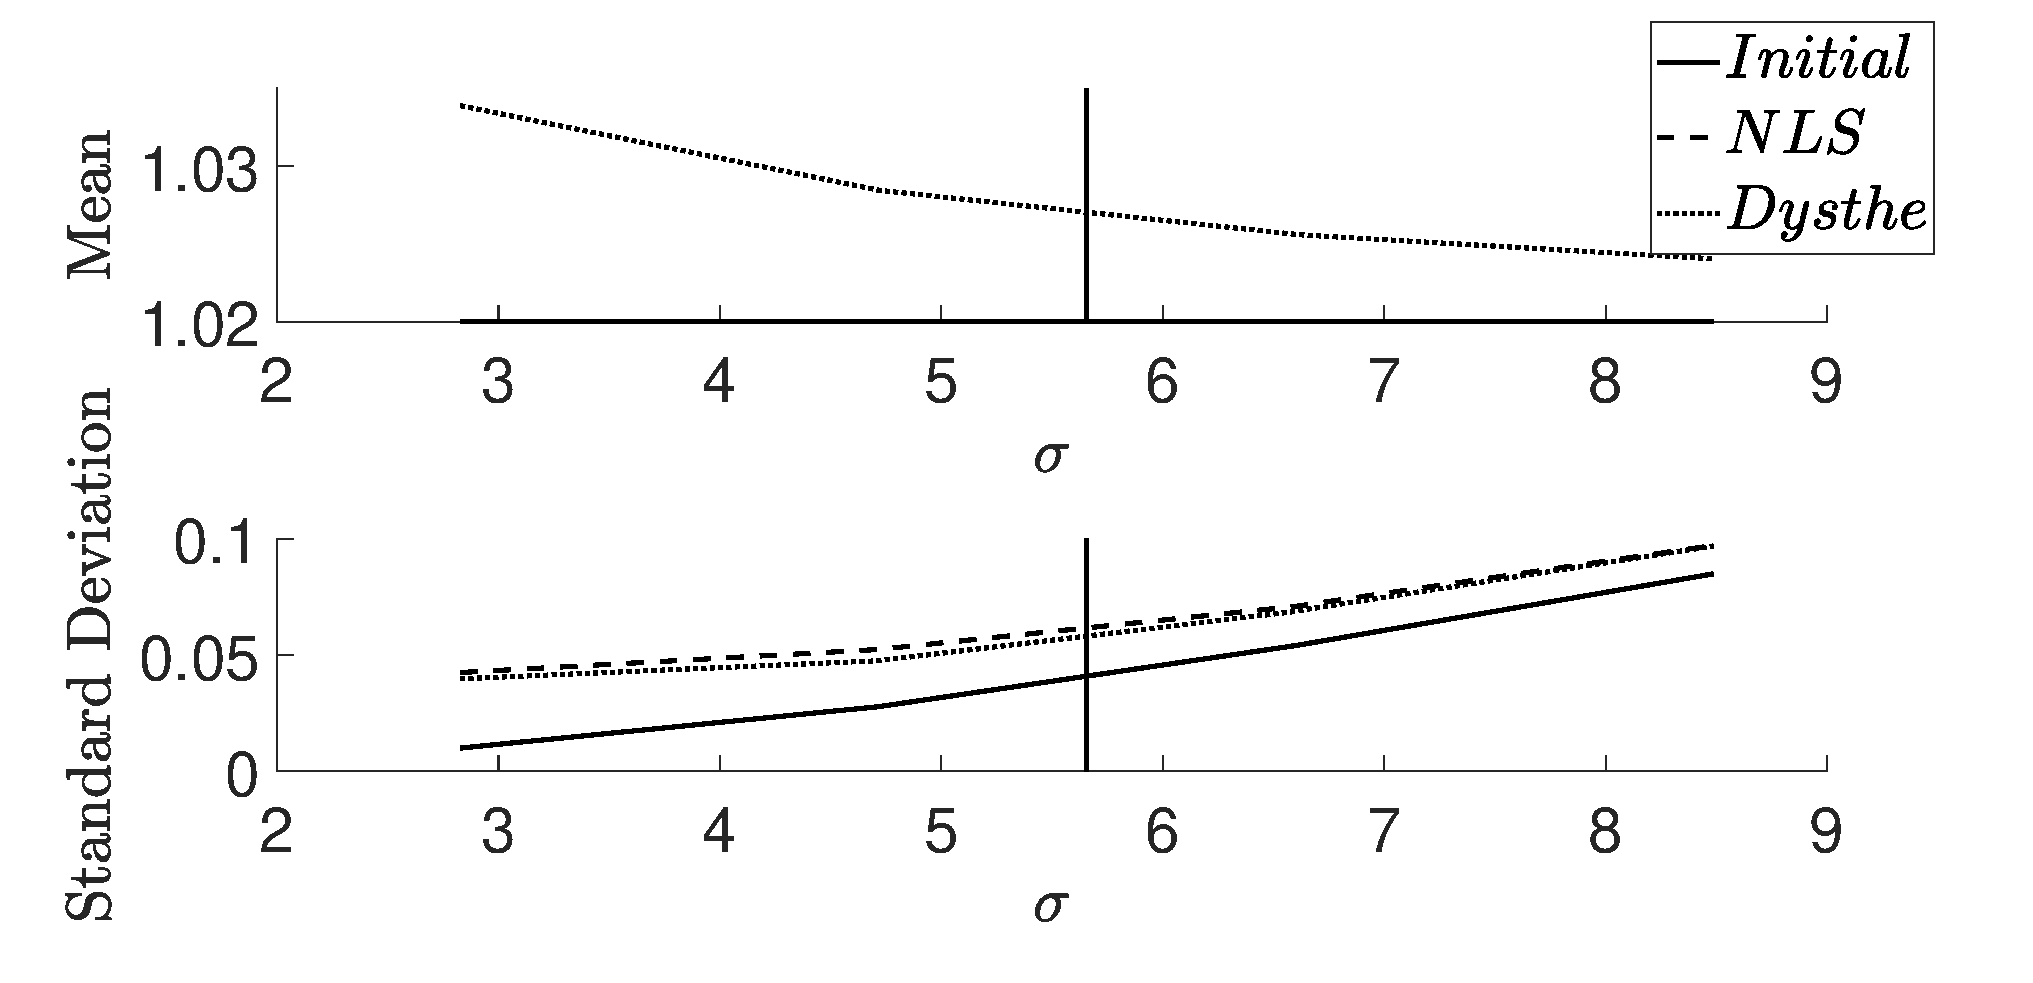
\includegraphics[width=.65\textwidth]{omega_0_mean_std_plot_ep_pt05}\\
(d) $\epsilon=.05$
\end{tabular}
\caption{For $\omega=0$, in (a) and (c) plots of the distributions for $\epsilon=.1$ and $\epsilon=.05$ respectively,  with $\sigma=1.05\sigma_{c}$.  In (b) and (d) comparison of the means and standard deviations between the initial averaged spectral density for $\epsilon=.1$ and $\epsilon=.05$ respectively.  The vertical line denotes the spectral width corresponding to the BFI condition.}
\label{fig:meanstdom0}
\end{figure}

\subsection*{Strong-Co Shear: $\omega = 1.12$}

Finally, by letting $\omega=1$, we further reduce the BFI threshold to $\sigma > 2.7$, opening up a yet wider range of stable initial conditions.  Likewise, the VDE dynamics are far more in line with those seen from the NLSE, even in the case that $\epsilon=.1$; see Figure \ref{fig:meanstdom1}.  Therefore, we see how vorticity propagating in the correct direction can vastly reduce the impact of MI, even in a far more nonlinear model like the VDE.  

\begin{figure}[!ht]
\centering
\begin{tabular}{c}
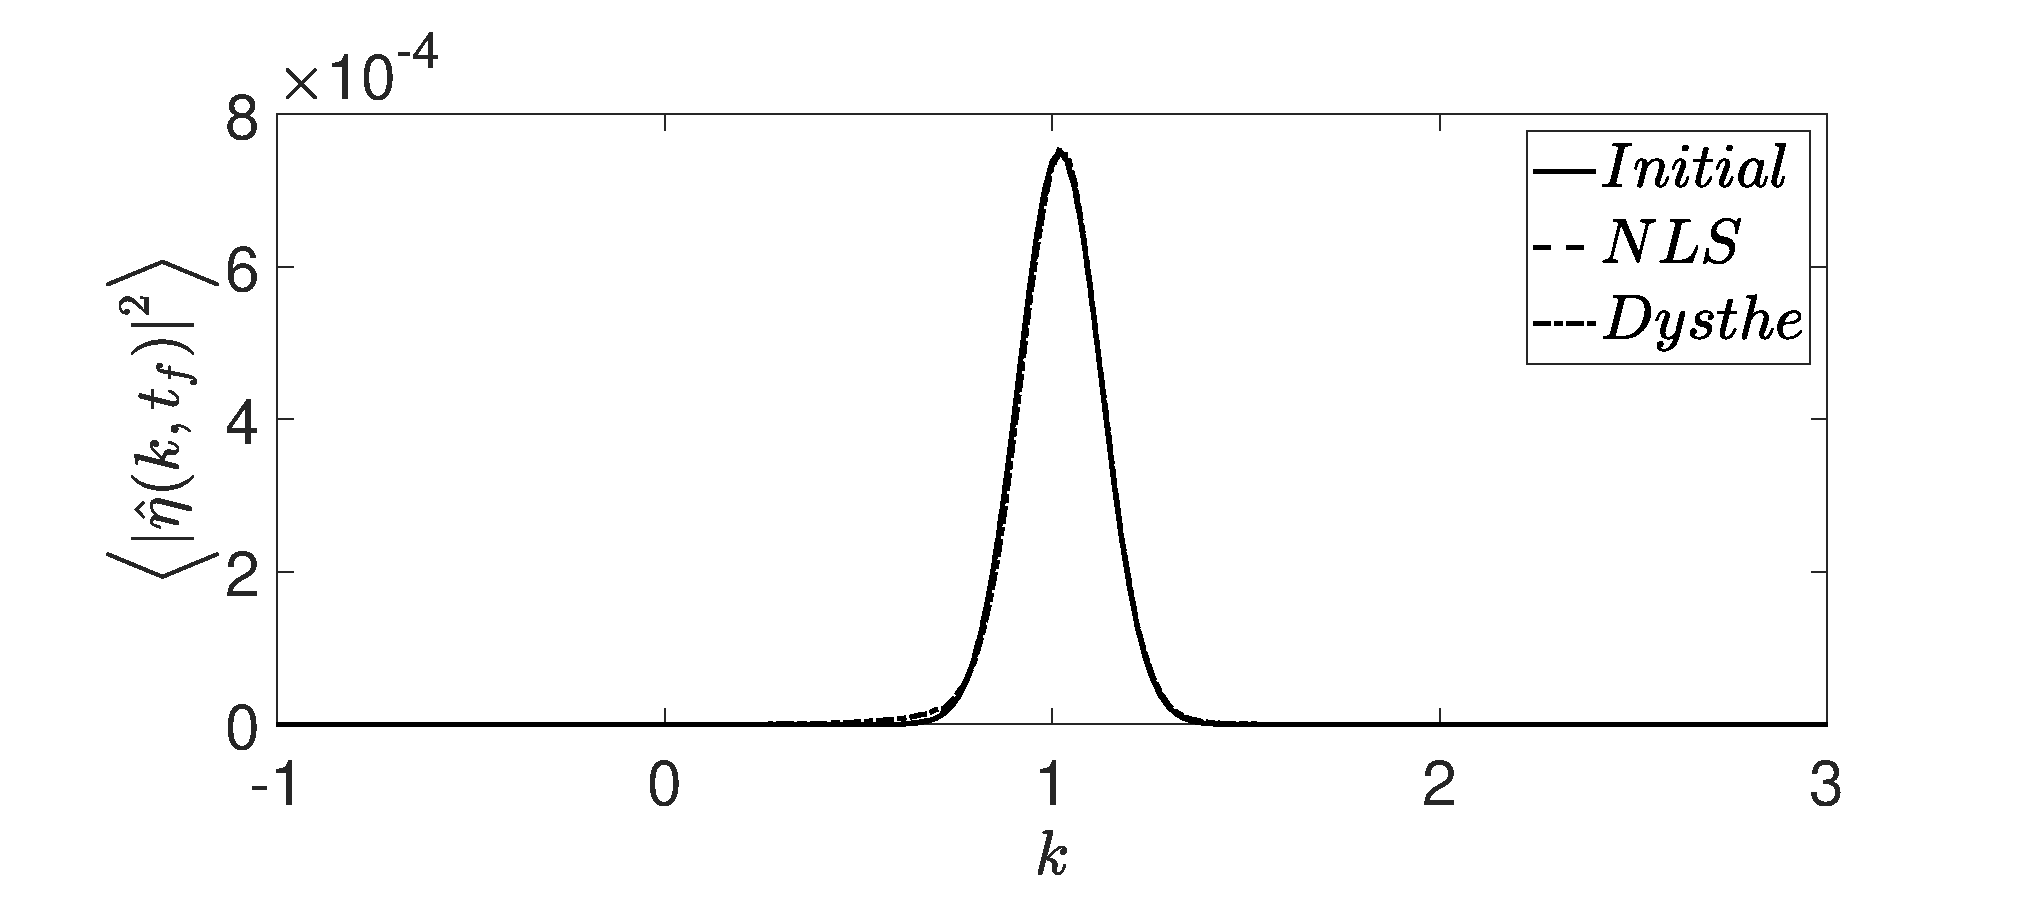
\includegraphics[width=.65\textwidth]{pdf_w_1pt12_ep_pt1_Nens_512} \\
(a) $\epsilon=.1$\\
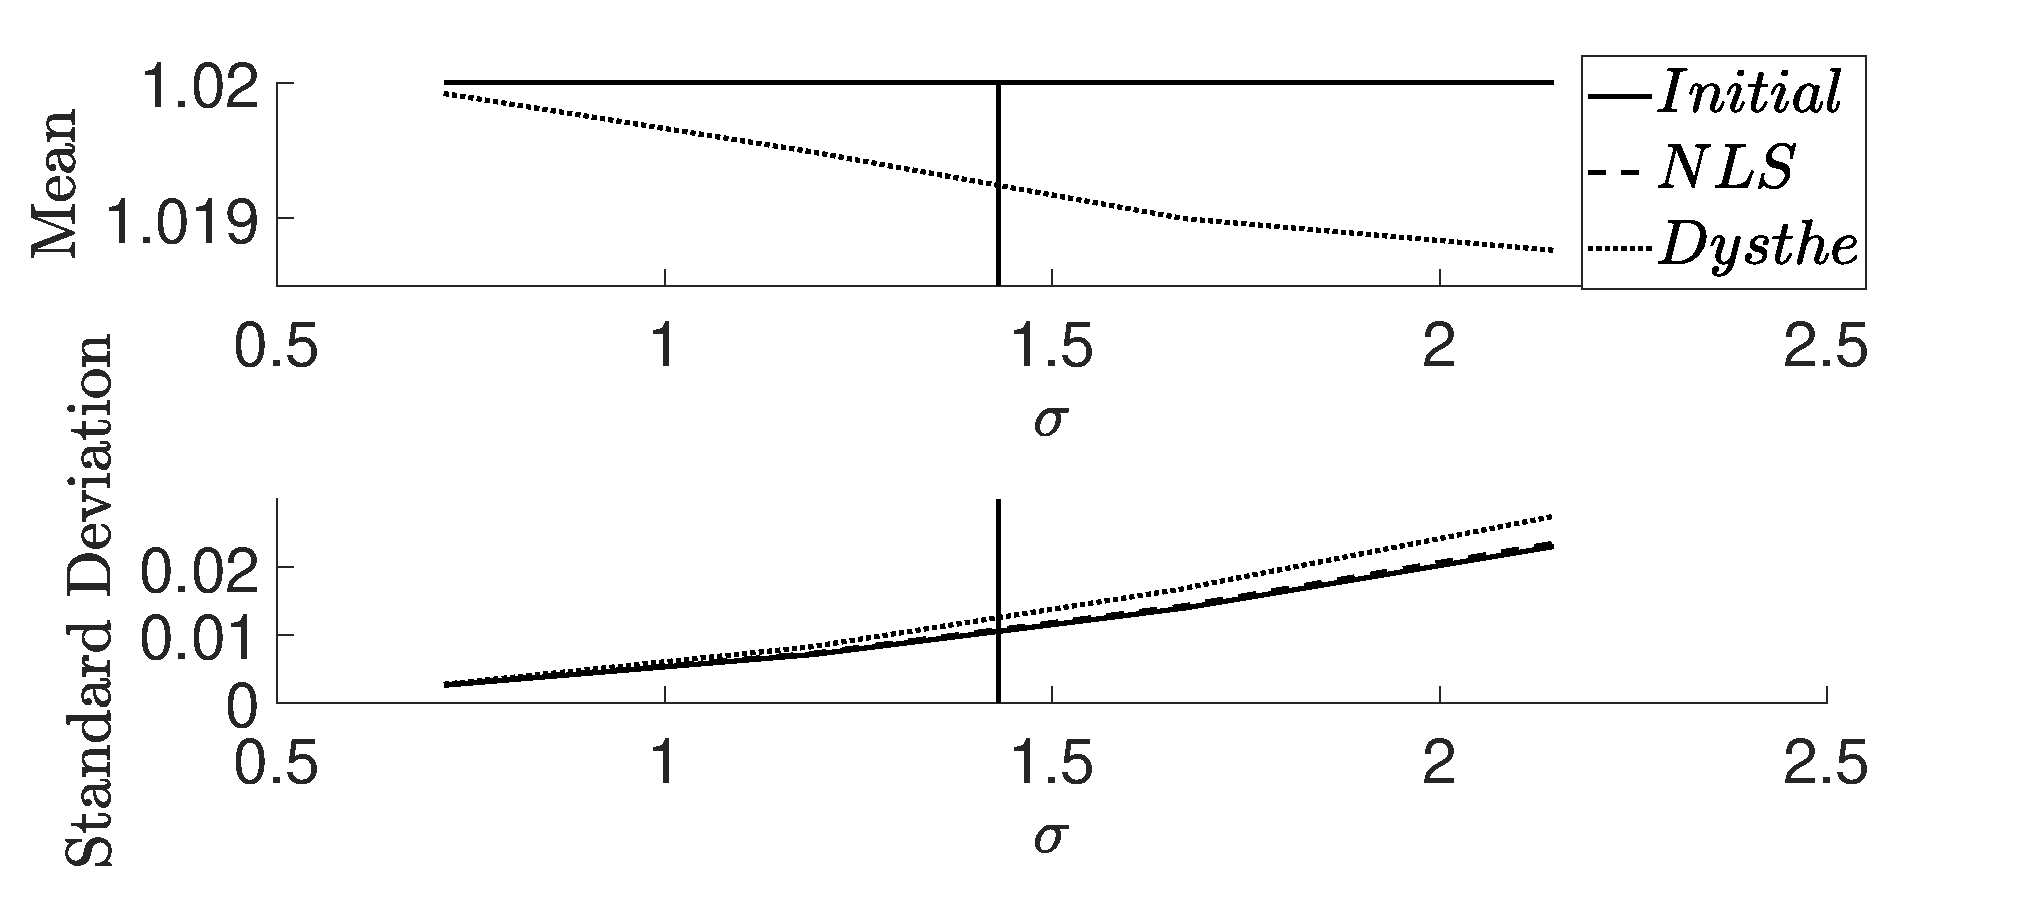
\includegraphics[width=.65\textwidth]{omega_1pt12_mean_std_plot_ep_pt1}\\
(b) $\epsilon=.1$ \\
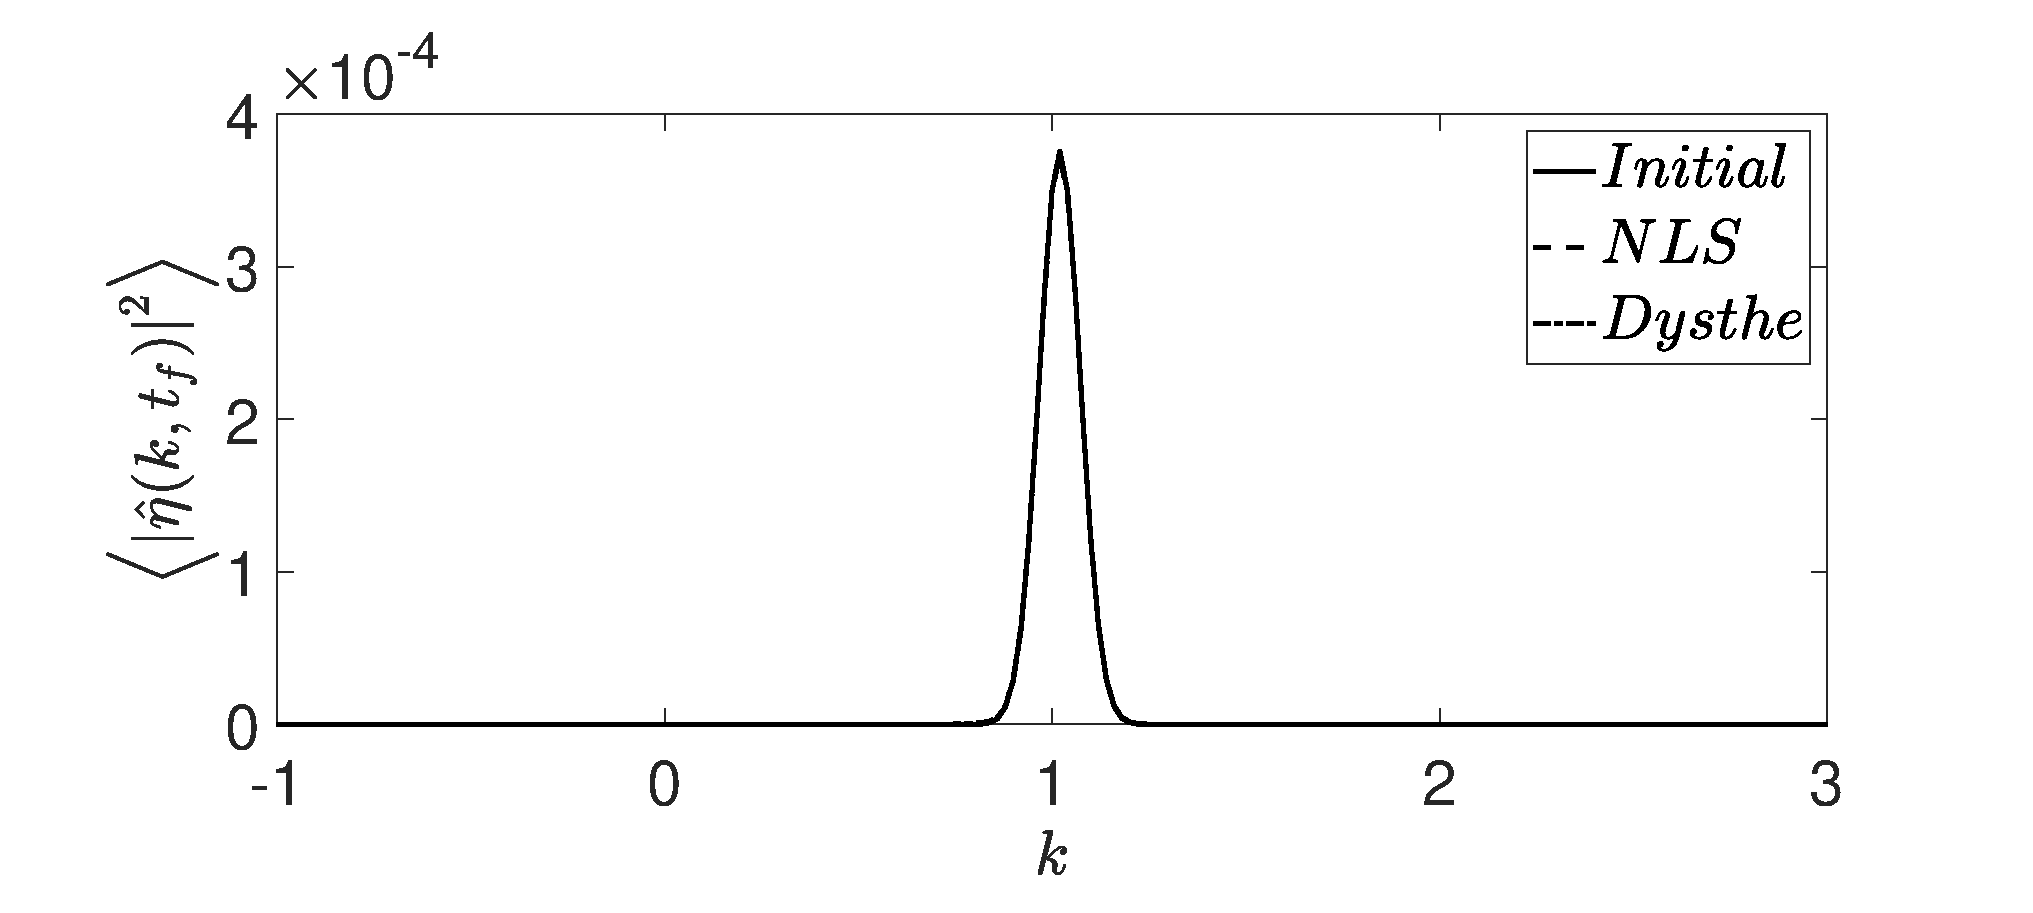
\includegraphics[width=.65\textwidth]{pdf_w_1pt12_ep_pt05_Nens_512}\\
(c) $\epsilon=.05$ \\
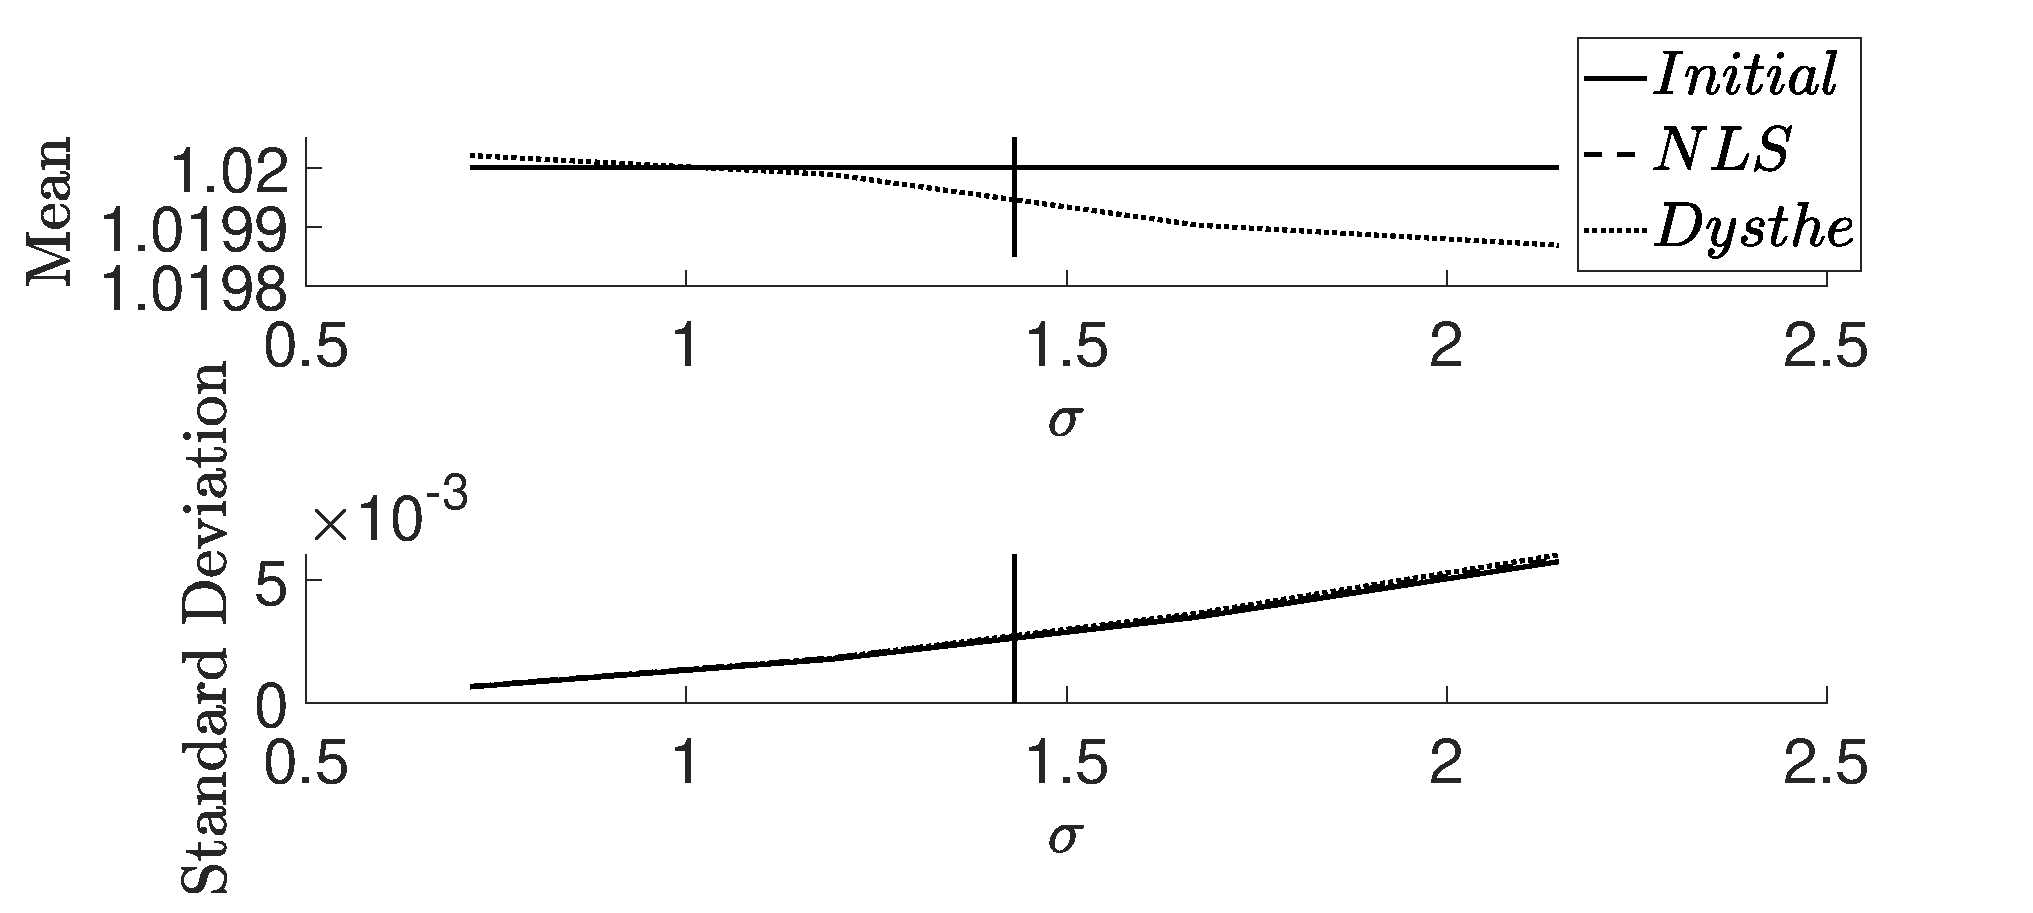
\includegraphics[width=.65\textwidth]{omega_1pt12_mean_std_plot_ep_pt05}\\
(d) $\epsilon=.05$
\end{tabular}
\caption{For $\omega=1.12$, in (a) and (c) plots of the distributions for $\epsilon=.1$ and $\epsilon=.05$ respectively,  with $\sigma=1.05\sigma_{c}$.  In (b) and (d) comparison of the means and standard deviations between the initial averaged spectral density for $\epsilon=.1$ and $\epsilon=.05$ respectively.  The vertical line denotes the spectral width corresponding to the BFI condition.}
\label{fig:meanstdom1}
\end{figure}

\section*{Conclusion}

In this work, we have studied the modulational stability of nearly modulated deep-water waves under the influence of steady linear shear profiles in the more physically realistic case in which the modulation is done on wave packets.  As we see, the vorticity profile has a strong influence on the stability properties of the wave train, with strong counter propagating shears exacerbating modulational instability effects.  In contrast, strong copropagating shears all but supress modulational instability.  Thus, we see vorticity effects can have significant implications for what the most likely observed deep water wavetrains are.  Likewise, in trying to interpret oceanographic data, vortical effects should be taken into account in modeling so as to be able to properly interpret observed data.    


\bibliography{deep_water_shear_Feb2}
\bibliographystyle{unsrt}
\end{document}